%% ============================================================
%%  Golden Substrate series -- canonical preamble.
%%  Identical across all papers except for \hypersetup{pdftitle=...}.
%% ============================================================

\documentclass[11pt,a4paper]{article}

\usepackage{amsmath,amssymb,amsthm}
\usepackage{mathtools}
\usepackage{geometry}
\usepackage{xcolor}

\definecolor{linkInternal}{HTML}{1F4E79}
\definecolor{linkExternal}{HTML}{2F5496}
\definecolor{linkCite}{HTML}{806600}
\usepackage[colorlinks=true,
            linkcolor=linkInternal,
            citecolor=linkCite,
            urlcolor=linkExternal,
            pdfborder={0 0 0},
            bookmarksnumbered=true,
            breaklinks=true]{hyperref}
\hypersetup{%
  pdfauthor={Kristin Tynski},
  pdftitle={The Metabolic Interpretation of FSCTF: Eating as the Creation Cycle (Paper V)},
  pdfsubject={Copyright (c) 2026 Kristin Tynski. All rights reserved.}%
}

\usepackage{cleveref}
\usepackage{booktabs}
\usepackage{array}
\usepackage{longtable}
\usepackage{enumitem}
\usepackage{lmodern}
\usepackage[T1]{fontenc}
\usepackage[protrusion=true,expansion=false]{microtype}
\usepackage{fancyhdr}
\usepackage[font=small,labelfont=bf,format=plain,labelsep=period]{caption}
\usepackage[framemethod=tikz]{mdframed}
\usepackage{tikz}
\usetikzlibrary{arrows.meta,positioning,calc,decorations.pathmorphing,shapes.geometric,fit,backgrounds,automata}

\geometry{margin=1in}
\setlength{\emergencystretch}{5em}

\theoremstyle{plain}
\newtheorem{theorem}{Theorem}[section]
\newtheorem{proposition}[theorem]{Proposition}
\newtheorem{lemma}[theorem]{Lemma}
\newtheorem{corollary}[theorem]{Corollary}
\newtheorem{conjecture}[theorem]{Conjecture}

\theoremstyle{definition}
\newtheorem{definition}[theorem]{Definition}
\newtheorem{axiom}[theorem]{Axiom}
\newtheorem{principle}[theorem]{Principle}

\theoremstyle{remark}
\newtheorem{remark}[theorem]{Remark}

\numberwithin{equation}{section}

%% --- Canonical notation (union across the series) ------------------
\providecommand{\Cl}{\mathrm{Cl}}
\providecommand{\GA}[2]{\mathbb{G}_{#1,#2}}
\providecommand{\R}{\mathbb{R}}
\providecommand{\C}{\mathbb{C}}
\providecommand{\Z}{\mathbb{Z}}
\providecommand{\Q}{\mathbb{Q}}
\providecommand{\N}{\mathbb{N}}
\providecommand{\F}{\mathbb{F}}
\providecommand{\HH}{\mathbb{H}}
\providecommand{\OO}{\mathbb{O}}
\providecommand{\Hh}{\mathbb{H}}
\providecommand{\Hp}{\mathbb{H}'}
\providecommand{\Os}{\mathbb{O}'}
\providecommand{\ZZ}{\mathbb{Z}}
\providecommand{\QQ}{\mathbb{Q}}
\providecommand{\RR}{\mathbb{R}}
\providecommand{\CC}{\mathbb{C}}
\providecommand{\FF}{\mathbb{F}}
\providecommand{\NN}{\mathbb{N}}
\providecommand{\Reals}{\mathbb{R}}
\providecommand{\Complex}{\mathbb{C}}
\providecommand{\Nat}{\mathbb{N}}
\providecommand{\Zp}{\ensuremath{\mathbb{Z}[\varphi]}}
\providecommand{\Qp}{\ensuremath{\mathbb{Q}(\sqrt{5})}}
\providecommand{\Gphi}{\ensuremath{\Gamma_{\varphi}}}
\providecommand{\E}{\mathbb{E}}
\providecommand{\PG}{\mathrm{PG}}

\providecommand{\vp}{\varphi}
\providecommand{\ps}{\psi}
\providecommand{\eps}{\varepsilon}
\providecommand{\half}{\tfrac{1}{2}}

\providecommand{\EF}{\mathcal{E}}
\providecommand{\PF}{\mathcal{P}}
\providecommand{\ZF}{\mathcal{Z}}
\providecommand{\W}{\mathcal{W}}
\providecommand{\cO}{\mathcal{O}}
\providecommand{\Lo}{\mathcal{L}}
\providecommand{\Lk}{L}

\providecommand{\fk}[1]{\mathfrak{#1}}
\providecommand{\fP}{\mathfrak{P}}
\providecommand{\fp}{\mathfrak{p}}
\providecommand{\slgo}{\mathfrak{sl}}
\providecommand{\sogo}{\mathfrak{so}}
\providecommand{\spgo}{\mathfrak{sp}}

\providecommand{\eb}[1]{e_{#1}}

\DeclareMathOperator{\Tr}{Tr}
\DeclareMathOperator{\Spec}{Spec}
\DeclareMathOperator{\Aut}{Aut}
\DeclareMathOperator{\Der}{Der}
\DeclareMathOperator{\End}{End}
\DeclareMathOperator{\Hom}{Hom}
\DeclareMathOperator{\Sym}{Sym}
\DeclareMathOperator{\Gal}{Gal}
\DeclareMathOperator{\Res}{Res}
\DeclareMathOperator{\BC}{BC}
\DeclareMathOperator{\Frob}{Frob}
\DeclareMathOperator{\Nm}{N}
\DeclareMathOperator{\Disc}{Disc}
\DeclareMathOperator{\disc}{disc}
\DeclareMathOperator{\Spin}{Spin}
\DeclareMathOperator{\Span}{span}
\DeclareMathOperator{\spn}{span}
\DeclareMathOperator{\rk}{rk}
\DeclareMathOperator{\Img}{Im}
\DeclareMathOperator{\im}{Im}
\DeclareMathOperator{\tr}{tr}
\DeclareMathOperator{\ad}{ad}
\DeclareMathOperator{\sgn}{sgn}
\providecommand{\PSL}{\operatorname{PSL}}
\providecommand{\SL}{\operatorname{SL}}
\providecommand{\GL}{\operatorname{GL}}
\providecommand{\id}{\mathrm{id}}

\providecommand{\Ephi}{\mathcal{E}_{\vp}}
\providecommand{\Pf}{P_4}
\providecommand{\Qf}{Q_4}
\providecommand{\seamfix}{\mathrm{seam\_fix}}
\providecommand{\seamtwist}{\mathrm{seam\_twist}}

\definecolor{accentBlue}{HTML}{2F80ED}
\definecolor{accentGray}{HTML}{6B7C93}
\definecolor{accentMuted}{HTML}{D5DBE0}

\newmdenv[
  linecolor=accentBlue!50,
  linewidth=0.6pt,
  backgroundcolor=accentBlue!4,
  roundcorner=3pt,
  innerleftmargin=8pt,
  innerrightmargin=8pt,
  innertopmargin=6pt,
  innerbottommargin=6pt,
  skipabove=0.8em,
  skipbelow=0.8em,
]{keyresultbox}

\newmdenv[
  linecolor=accentGray!25,
  linewidth=0.5pt,
  backgroundcolor=accentGray!5,
  roundcorner=2.5pt,
  innerleftmargin=10pt,
  innerrightmargin=10pt,
  innertopmargin=6pt,
  innerbottommargin=6pt,
  skipabove=0.6em,
  skipbelow=1.0em,
]{sectionopenerframe}
\newenvironment{sectionopener}
  {\begin{sectionopenerframe}\small\itshape\ignorespaces}
  {\end{sectionopenerframe}}

\pagestyle{fancy}
\fancyhf{}
\renewcommand{\headrulewidth}{0pt}
\fancyhead[L]{\small\itshape\color{accentGray}\nouppercase{\leftmark}}
\fancyhead[R]{\small\color{accentGray}\thepage}
\fancyfoot[C]{}
\renewcommand{\sectionmark}[1]{\markboth{\thesection.\ #1}{}}

\widowpenalty=1000
\clubpenalty=1000
\setlength{\parskip}{0.55em plus 0.2em minus 0.05em}
\setlength{\parindent}{1.2em}
\AtBeginEnvironment{itemize}{\setlength{\parskip}{0pt}}
\AtBeginEnvironment{enumerate}{\setlength{\parskip}{0pt}}
\AtBeginEnvironment{description}{\setlength{\parskip}{0pt}}

\title{The Metabolic Interpretation of FSCTF:\\
Eating as the Creation Cycle\\[4pt]
{\large Paper V in the FSCTF series}}

\author{Kristin Tynski}
\date{May 2026 \\[6pt] {\small\textcopyright\ 2026 Kristin Tynski. All rights reserved.}}

\begin{document}

\thispagestyle{empty}
\maketitle

\begin{center}
{\color{accentMuted}\rule{0.55\textwidth}{0.5pt}}
\end{center}

\begin{center}
\footnotesize
\textbf{MSC 2020:} 15A66 (Primary); 17A35, 81R25, 92C40, 68Q70 (Secondary).\\
\textbf{Keywords:} Clifford algebra, Peirce decomposition, idempotents, nilpotents,
metabolism, FSCTF, signature duality, finite-state transducers,
boundary-preserving dynamics.\\
\textbf{Code:} \texttt{genesis-simulation/dynamics/metabolic.js},
\texttt{genesis-simulation/tests/test-metabolic-theory.mjs}
(53 tests, zero failures).
\end{center}
\vspace{0.4em}
\begin{center}
{\color{accentMuted}\rule{0.55\textwidth}{0.5pt}}
\end{center}

\begin{abstract}
\noindent
The FSCTF creation cycle $R = G(W(L(\Omega)))$ admits a precise
metabolic reading: every digestion is the equation running on
external matter with the witness as invariant. This paper makes the
reading mathematical. We show that the four phases of metabolism
(ingestion, digestion, absorption, excretion) correspond bijectively
to four algebraic operations in the Clifford algebra $\Cl(3,1)$, that
the digestive seam is the Peirce cross-sector of a primitive idempotent
split, and that the difference between devouring and communion is
parameterized by a single integer (the number of Grace contraction
steps). Eleven theorems, each independently verifiable by short
numerical script, establish the framework rigorously: seven core
theorems on the metabolic cycle plus four pathology theorems
(autoimmunity, immunodeficiency, microbiome, constipation) that
originated as biological predictions and are here promoted to
pure algebra. The paper makes no claims to novelty in the underlying
algebra: everything reduces to operations already present in the
substrate of Paper~I. The contribution is the bijection, the
identification of two distinct witness invariants, the closed-form
decay law $c_k(t) = c_k(0) \exp(-t(1 - \vp^{-k}))$ for grade-$k$
Grace dynamics, and four algebraic pathology theorems with explicit
biological readings.

\medskip\noindent\textbf{Three load-bearing results.}

\medskip\noindent\textbf{(M1) The metabolic cycle is the creation
cycle.} \emph{(\cref{thm:cycle,cor:phase-bijection}.)} The map
\[
(\text{ingest}, \text{digest}, \text{absorb}+\text{metabolize}, \text{excrete})
\longleftrightarrow
(M + \lambda I, \mathrm{decompose}, G^n, \mathrm{mixed} - \mathrm{reconstruct})
\]
is a bijection of operational primitives in $\Cl(3,1)$. The composition
satisfies energy conservation
$\mathrm{absorbed} + \mathrm{residue} = \mathrm{mixed}$ exactly.

\medskip\noindent\textbf{(M2) Grace decay is closed-form
grade-diagonal.} \emph{(\cref{thm:decay}.)} Under the Grace
contraction $G : \R^{16} \to \R^{16}$ given by $G(c)_i = \vp^{-\mathrm{grade}(e_i)} c_i$
in any orthonormal grade basis,
\[
c_k(t) = c_k(0) \cdot \exp\!\big(-t(1 - \vp^{-k})\big), \qquad k \in \{0,1,2,3,4\}.
\]
The grade-$0$ (scalar witness) coefficient is the unique fixed point;
the pseudoscalar (grade $4$) decays fastest. Verified to $10^{-10}$.

\medskip\noindent\textbf{(M3) Two distinct witness invariants.}
\emph{(\cref{thm:two-witnesses}.)} The scalar coefficient $c_0$ is the
eigenmode-$1$ of $\mathrm{graceContract}$ in coefficient space, while
the matrix row $M[0,{:}]$ is the eigenmode-$1$ of $\mathrm{masterStep}$
in matrix space. \emph{Neither preserves the other's invariant.}
This distinction was implicit in the existing simulation code and
is made explicit here. It resolves an ambiguity in
EverythingFromWitness §4.

\medskip\noindent\textbf{Scope.} All proofs reduce to closed-form
algebra in $\Cl(3,1) \cong M_4(\R)$. The framework is a
re-reading, not a new physics; its empirical content lies in
specific biological predictions stated in §\ref{sec:predictions}.
\end{abstract}

\medskip
\noindent\textbf{What this paper does.}
\begin{itemize}[leftmargin=1.5em,nosep,topsep=2pt]
  \item Reads the FSCTF creation cycle
        $R = G(W(L(\Omega)))$ as a \emph{metabolic} interpretation
        of the substrate: opening Grace, decomposing food
        (Sacrifice), retaining the boundary-preserving residue.
  \item Encodes healthy and pathological eating as accepted vs.\
        rejected sequences on a $64$-state braid-grammar
        finite-state transducer over the alphabet $\{W,G,S,C,L,P,X\}$;
        proves the accepting depths are exactly $\{2,3,4,7\}$.
  \item Derives four \emph{pathology theorems}
        -- autoimmunity, immunodeficiency, microbiome transport,
        constipation -- as failure modes of the same boundary
        algebra that underwrites the substrate.
\end{itemize}

\medskip
\noindent\textbf{Place in the series.}
This is the \emph{operational/biological} side paper for the
main trilogy (I~$\to$~II~$\to$~III).  It depends on Paper~I
(Clifford algebra, Peirce idempotents) and Paper~III (monad/braid
grammar) but is independent of Papers~II, VI, VII, and VIII.

\tableofcontents
\clearpage

%% =====================================================================
\section{Introduction}
\label{sec:intro}
%% =====================================================================

\begin{sectionopener}
This paper takes a sentence from natural language --- ``eating is asymmetric
coherence transfer across a boundary'' --- and shows that it has a
unique algebraic realization in the substrate of Paper~I. The
realization makes seven testable numerical claims, all of which we
verify, and four biological predictions, which we state but do not
verify.
\end{sectionopener}

\subsection*{The question}

What is eating?

The biological answer (a system imports matter, decomposes it,
absorbs compatible structure, rejects incompatible residue) is
operational but underdetermines the formalism. We ask: under
which choice of algebraic primitives does the operational answer
become unique?

The answer, given a Clifford algebra $\Cl(3,1)$ over $\R$ with
primitive idempotents and a contraction operator $G$ satisfying the
Lyapunov property of Paper~I, is exactly one. The bijection is
forced by:

\begin{enumerate}[label=(\arabic*)]
\item Energy conservation across the cycle (forces excretion as
  exact residue, not as decay).
\item Witness invariance through ingestion (forces absorption to be
  a Grace-stable projection).
\item Boundary-status (not geometric) interior/exterior (forces the
  digestive surface to be the Peirce cross-sector of an idempotent
  split, not a geometric boundary).
\item Single-parameter dial between devouring and communion (forces
  the parameter to be the integer Grace step count $n$).
\end{enumerate}

\subsection*{The bijection}

\begin{center}
\begin{tabular}{ll}
\toprule
\textbf{Metabolic phase} & \textbf{Algebraic operation} \\
\midrule
ingestion & $\mathrm{mixed} = \mathrm{self} + \lambda \cdot \mathrm{input}$ \\
digestion & $c = \mathrm{decompose}(\mathrm{mixed})$ \\
absorption + metabolism & iterated Grace: $c \mapsto G^n(c)$ \\
excretion & $\mathrm{residue} = \mathrm{mixed} - \mathrm{reconstruct}(G^n(c))$ \\
\bottomrule
\end{tabular}
\end{center}

\subsection*{Relation to Papers I--IV}

This paper depends on Paper~I for the algebraic substrate
($\Cl(3,1)$, the Grace contraction, the idempotent split). It does
not depend on Papers II--IV. The metabolic reading is a new
interpretive layer over the existing substrate; no new algebra
is introduced.

%% =====================================================================
\section{Preliminaries}
\label{sec:prelim}
%% =====================================================================

We assume the reader is familiar with the substrate of Paper~I and
state only what is needed.

\subsection{The algebra}

Let $V = \R^4$ with the metric of signature $(3,1)$, basis
$\{\gamma_0, \gamma_1, \gamma_2, \gamma_3\}$ satisfying
$\gamma_0^2 = -1$, $\gamma_i^2 = +1$ for $i = 1,2,3$. The Clifford
algebra $\Cl(3,1)$ is $16$-dimensional over $\R$ and isomorphic to
$M_4(\R)$. We work in this isomorphism throughout, representing
elements as $4 \times 4$ real matrices.

The grade decomposition is
\[
\Cl(3,1) = \Lambda^0 \oplus \Lambda^1 \oplus \Lambda^2 \oplus \Lambda^3 \oplus \Lambda^4,
\]
with grade dimensions $(1, 4, 6, 4, 1)$. An element $M$ has
coefficients $c = (c_0, \ldots, c_{15})$ in any chosen grade-ordered
basis.

\subsection{The primitive idempotents}

Let $\Pf, \Qf \in \Cl(3,1)$ be the primitive idempotent pair from
Paper~I, with $\Pf + \Qf = I$ and $\Pf\Qf = \Qf\Pf = 0$. In the
matrix representation chosen here,
\[
\Pf = \tfrac{1}{4}\,\mathrm{diag}(4, 0, 0, 0) = E_{00}, \qquad
\Qf = \tfrac{1}{4}\,\mathrm{diag}(0, 4, 4, 4) = I - E_{00},
\]
where $E_{ij}$ is the standard matrix unit. We have rescaled the
representation so $\Pf$ and $\Qf$ are exact projections.

The Peirce decomposition of any $M \in \Cl(3,1)$ is
\begin{equation}
\label{eq:peirce}
M = \underbrace{\Pf M \Pf}_{M_{pp}} \;+\; \underbrace{\Pf M \Qf + \Qf M \Pf}_{O(M)} \;+\; \underbrace{\Qf M \Qf}_{M_{qq}}.
\end{equation}

\subsection{The Grace operator}

The Grace contraction $G : \R^{16} \to \R^{16}$ acts diagonally in
the grade basis:
\begin{equation}
\label{eq:grace}
G(c)_i = \vp^{-\mathrm{grade}(e_i)} \, c_i.
\end{equation}
Equivalently, $G$ has eigenvalues $\{1, \vp^{-1}, \vp^{-2}, \vp^{-3}, \vp^{-4}\}$
with multiplicities $(1, 4, 6, 4, 1)$.

When the Grace coupling $\kappa = 2\vp^{-3}$ governs continuous
dynamics, the per-step contraction reads (after the convention
fixed in Paper~I) $c_i \mapsto e^{-(1 - \vp^{-\mathrm{grade}(e_i)})} c_i$
under unit time step. We use this convention.

\subsection{The Love operator}

The Love unfolding $L : \R^{16} \to \R^{16}$ injects grade-$1$
content from the witness sector. It satisfies $L(c)_k = c_k$ for
$k \notin \{1,2,3,4\}$ (grade $1$) and adds a witness-coupled
contribution in grades $1$ and $3$ (odd grades).

\subsection{The master step}

The combined dynamics is $M \mapsto S(M)$ where $S$ is the
matrix-level update of Paper~III §2. $S$ preserves the first matrix
row $M[0, {:}]$ exactly (verified numerically; we restate this
below as \cref{thm:two-witnesses}).

%% =====================================================================
\section{The Metabolic Cycle}
\label{sec:cycle}
%% =====================================================================

\begin{definition}[Metabolic cycle]
\label{def:cycle}
Given $\mathrm{self}, \mathrm{input} \in \Cl(3,1)$, an ingestion
scale $\lambda \in \R_{>0}$, and a number of Grace steps $n \in \N$,
the \emph{metabolic cycle} is the four-tuple
\[
\big(\mathrm{mixed},\; c,\; \mathrm{absorbed},\; \mathrm{residue}\big)
\]
where
\begin{align*}
\mathrm{mixed} &= \mathrm{self} + \lambda \cdot \mathrm{input}, \\
c &= \mathrm{decompose}(\mathrm{mixed}) \in \R^{16}, \\
\mathrm{absorbed} &= \mathrm{reconstruct}\big(G^n(c)\big) \in \Cl(3,1), \\
\mathrm{residue} &= \mathrm{mixed} - \mathrm{absorbed}.
\end{align*}
\end{definition}

\begin{theorem}[Energy conservation]
\label{thm:cycle}
For every $\mathrm{self}, \mathrm{input}, \lambda, n$,
\[
\mathrm{absorbed} + \mathrm{residue} = \mathrm{mixed}
\]
exactly. Equivalently, the metabolic cycle preserves total matter
to machine precision.
\end{theorem}

\begin{proof}
$\mathrm{residue}$ is defined as $\mathrm{mixed} - \mathrm{absorbed}$.
\end{proof}

\begin{corollary}[Phase bijection]
\label{cor:phase-bijection}
The bijection
\[
\begin{array}{rcl}
\text{ingestion} &\longleftrightarrow& M + \lambda I \\
\text{digestion} &\longleftrightarrow& \mathrm{decompose} \\
\text{absorption} + \text{metabolism} &\longleftrightarrow& G^n \\
\text{excretion} &\longleftrightarrow& \mathrm{mixed} - \mathrm{reconstruct}
\end{array}
\]
is forced by simultaneous satisfaction of (i) energy conservation,
(ii) witness invariance, (iii) boundary-status interior/exterior,
(iv) single-parameter devouring--communion dial.
\end{corollary}

\begin{proof}
Each condition eliminates an alternative formulation. (i) excludes
``absorption as decay'' (which would lose matter). (ii) requires
the absorbed component to preserve the grade-$0$ coefficient, and
$G$ is the unique contraction with this property among
grade-diagonal operators. (iii) requires the digestive seam to be
algebraic (Peirce cross-sector), not geometric. (iv) requires a
discrete-step dial, and the integer Grace step count is the
minimal such.
\end{proof}

\subsection{Grace decay law}

\begin{theorem}[Closed-form Grace decay]
\label{thm:decay}
Under the convention $c \mapsto e^{-(1 - \vp^{-k})} c$ for grade-$k$
content,
\[
c_k(t) = c_k(0) \cdot \exp\!\big(-t(1 - \vp^{-k})\big),
\qquad t \in \N,\; k \in \{0,1,2,3,4\}.
\]
\end{theorem}

\begin{proof}
$G$ is diagonal in the grade basis with eigenvalue $\vp^{-k}$ on
grade $k$; the convention rewrites this as $e^{-(1 - \vp^{-k})}$.
Iteration yields $G^t$ with eigenvalue $e^{-t(1 - \vp^{-k})}$.
\end{proof}

\begin{corollary}[Decay rate table]
\label{cor:rates}
\[
\begin{array}{c|c}
\text{grade } k & \text{decay rate } 1 - \vp^{-k} \\
\hline
0 & 0.000\ldots \\
1 & 0.382\ldots \\
2 & 0.618\ldots \\
3 & 0.764\ldots \\
4 & 0.854\ldots \\
\end{array}
\]
The pseudoscalar (chiral history) decays fastest; the scalar
(witness) is fixed. This is the algebraic statement of ``the
witness persists through the flow.''
\end{corollary}

\begin{remark}
The rates are $1, 2\vp^{-2}, \vp^{-2}+\vp^{-3}, \ldots$ but the
closed-form $1 - \vp^{-k}$ is the cleanest expression. The
appearance of all five integer powers of $\vp$ in a single
spectrum is the structural reason Grace is unique up to the
golden-ratio scaling fixed in Paper~I.
\end{remark}

%% =====================================================================
\section{The Two Witness Invariants}
\label{sec:two-witnesses}
%% =====================================================================

\begin{theorem}[Two distinct witnesses]
\label{thm:two-witnesses}
Let $S$ be the master step of Paper~III and $G$ the Grace
contraction. Then:
\begin{enumerate}[label=(\roman*)]
\item For every $c \in \R^{16}$, $\big(G(c)\big)_0 = c_0$. The
  scalar coefficient is preserved by Grace.
\item For every $M \in \Cl(3,1)$, $\big(S(M)\big)[0,j] = M[0,j]$
  for $j = 0, 1, 2, 3$. The first matrix row is preserved by the
  master step.
\item Neither (i) nor (ii) implies the other: $S$ generically
  changes $c_0$ (because the trace of $S(M)$ differs from the trace
  of $M$), and $G$ generically changes $M[0,j]$ (because the
  pseudoscalar matrix has nonzero $[0, j]$ entries for $j \ne 0$).
\end{enumerate}
\end{theorem}

\begin{proof}
(i) is immediate from \eqref{eq:grace} since $\mathrm{grade}(e_0) = 0$.
(ii) is verified by direct inspection of $S$'s matrix
representation (Paper~III §2). For (iii): the trace
$\tr(M) = 4 c_0$ in our representation, and $S$ contracts off-diagonal
entries while modifying the diagonal trace by a Grace factor, hence
$c_0$ is not generically fixed by $S$. Conversely, the pseudoscalar
basis element $I_{(3,1)} = \gamma_0\gamma_1\gamma_2\gamma_3$ has
nonzero $[0,j]$ entries in the matrix representation, so a state
with pseudoscalar coefficient $c_{15} \ne 0$ has $M[0,j] \ne 0$,
and $G$ scales $c_{15}$ by $\vp^{-4} \ne 1$, changing $M[0,j]$.
\end{proof}

\begin{remark}
Previous notes (EverythingFromWitness §4) referred to ``the
witness invariant'' without disambiguating these two notions.
This paper fixes the distinction. The \emph{algebraic} witness is
$c_0$; the \emph{geometric} witness is $M[0,:]$. Both are stable
under their respective dynamics; neither under both.
\end{remark}

%% =====================================================================
\section{The Sealed Manifold and the Metabolic Seam}
\label{sec:seal}
%% =====================================================================

\begin{definition}[Sealed state]
\label{def:sealed}
A state $M \in \Cl(3,1)$ is \emph{sealed} if its Peirce cross-sector
$O(M)$ from \eqref{eq:peirce} vanishes. Equivalently,
\[
\mathrm{peirceTransport}(M) := \sqrt{\sum_{j=1}^{3}\!\big(M[0,j]^2 + M[j,0]^2\big)} \;=\; 0.
\]
\end{definition}

\begin{theorem}[Sealed predicate equivalence]
\label{thm:sealed}
The following are equivalent for $M \in \Cl(3,1)$ represented as a
$4 \times 4$ real matrix in the basis fixing $\Pf = E_{00}$:
\begin{enumerate}[label=(\roman*)]
\item $M$ is sealed.
\item $M = \Pf M \Pf + \Qf M \Qf$.
\item $M$ is block-diagonal with blocks $M[0,0]$ and $M[1{:}4, 1{:}4]$.
\end{enumerate}
\end{theorem}

\begin{proof}
$\Pf M \Pf = E_{00} M E_{00}$ has only $M[0,0]$ surviving;
$\Qf M \Qf = (I - E_{00}) M (I - E_{00})$ has only the
$M[1{:}4, 1{:}4]$ block surviving. The off-block content is
$\Pf M \Qf + \Qf M \Pf = E_{00} M (I - E_{00}) + (I - E_{00}) M E_{00}$,
which consists exactly of the entries $\{M[0,j], M[j,0] : j = 1, 2, 3\}$.
This vanishes iff $\mathrm{peirceTransport}(M) = 0$.
\end{proof}

\begin{proposition}[Pure scalar is sealed]
\label{prop:scalar-sealed}
For $c = (1, 0, \ldots, 0)$, the reconstruction is the identity
matrix $I_4$, which is sealed.
\end{proposition}

\begin{proof}
$I_4[0,j] = I_4[j,0] = 0$ for $j = 1, 2, 3$.
\end{proof}

\begin{theorem}[Love breaks the seal in one step]
\label{thm:love-breaks-seal}
Let $W = c_0 I_4$ be a pure witness state (sealed). Then after one
application of the Love operator $L$, the resulting state has
$\mathrm{peirceTransport} > 0$.
\end{theorem}

\begin{proof}
$L$ injects content into grades $1$ and $3$. The grade-$1$ basis
elements $\{\gamma_0, \gamma_1, \gamma_2, \gamma_3\}$ all have
nonzero off-diagonal entries in row $0$ or column $0$ in the
matrix representation (specifically, $\gamma_0 = -E_{00}$ has
purely diagonal entries, but $\gamma_1, \gamma_2, \gamma_3$ each
have nontrivial $[0, j]$ or $[j, 0]$ content). Since the Love
coupling is nonzero on at least one of $\gamma_1, \gamma_2, \gamma_3$,
the resulting state has nonzero Peirce cross-sector.
\end{proof}

\begin{remark}
\cref{thm:love-breaks-seal} is the algebraic content of the
statement ``hunger differentiates.'' A purely sealed witness has no
metabolism (no boundary, no exchange). Love is the operator that
creates a boundary; Grace is what preserves it under transformation.
\end{remark}

%% =====================================================================
\section{Devouring vs.\ Communion}
\label{sec:devouring}
%% =====================================================================

\begin{definition}[Devouring vs.\ communion]
\label{def:dvc}
With reference to the metabolic cycle of \cref{def:cycle}:
\begin{itemize}
\item \emph{Devouring} is the case $n = 0$ (no Grace steps).
\item \emph{Communion} is the asymptotic case $n \to \infty$.
\end{itemize}
\end{definition}

\begin{theorem}[Devouring--communion limits]
\label{thm:dvc-limits}
For the cycle of \cref{def:cycle}:
\begin{enumerate}[label=(\roman*)]
\item \textbf{Devouring.} If $n = 0$ then $\mathrm{absorbed} = \mathrm{mixed}$
  and $\mathrm{residue} = 0$. The self is fully contaminated by the
  input.
\item \textbf{Communion.} As $n \to \infty$, $\mathrm{absorbed}$
  converges to $c_0^{\mathrm{mixed}} I_4$ (the grade-$0$
  projection), and $\mathrm{residue}$ converges to the sum of all
  grade-$\geq 1$ content of $\mathrm{mixed}$.
\end{enumerate}
\end{theorem}

\begin{proof}
(i) At $n = 0$, $G^0$ is the identity, so $\mathrm{absorbed} = \mathrm{mixed}$.
(ii) From \cref{thm:decay}, $G^t$ has eigenvalue $e^{-t(1-\vp^{-k})}$
on grade $k$. For $k = 0$, this is $1$ for all $t$. For $k \geq 1$,
$1 - \vp^{-k} > 0$, so the eigenvalue tends to $0$ as $t \to \infty$.
Hence $G^t(c) \to c_0 \, \delta_0$ (only grade-$0$ survives), and
$\mathrm{reconstruct}(G^t(c)) \to c_0 I_4$. The residue is the
complement.
\end{proof}

\begin{corollary}[The single dial]
The transition from devouring to communion is monotonic in $n$:
$\|\mathrm{residue}\|$ is monotonically increasing in $n$, and
$\|\mathrm{absorbed} - c_0^{\mathrm{mixed}} I_4\|$ is monotonically
decreasing in $n$.
\end{corollary}

\begin{remark}[Pathology]
Three failure modes are distinguishable in this framework:
\begin{itemize}
\item \emph{Anorexia.} $\lambda = 0$ (no ingestion).
  $\mathrm{residue} = 0$ for trivial reason.
\item \emph{Toxicity.} Iterated ingestion with insufficient $n$.
  Grade-$\geq 1$ content accumulates; $\|\mathrm{self}\|$ grows
  monotonically without bound.
\item \emph{Constipation.} Excretion blocked. From the throat
  architecture of Paper~IV (mushrooms.md), if $P_\mathrm{clear} = 0$
  or $P_\mathrm{cap} = 0$, then total flux $J = 0$, and residue
  accumulates internally.
\end{itemize}
\end{remark}

%% =====================================================================
\section{Signature Duality as Metabolic Direction}
\label{sec:duality}
%% =====================================================================

The algebra $\Cl(3,1)$ has a sibling $\Cl(1,3)$ obtained by flipping
the signature. The metabolic reading interprets the two signatures
as the two directions of metabolic flow.

\begin{definition}[Metabolic direction]
\label{def:direction}
The \emph{ingestion direction} is the forward Merkaba transport
$M \mapsto R M \tilde R$, where $R$ is the Merkaba rotor and $\tilde R$
its reverse. The \emph{excretion direction} is the reverse Merkaba
transport $M \mapsto \tilde R M R$.
\end{definition}

\begin{theorem}[Directional asymmetry]
\label{thm:merkaba-asymmetry}
For generic $M \in \Cl(3,1)$ and generic Merkaba rotor $R$,
\[
R M \tilde R \;\ne\; \tilde R M R.
\]
\end{theorem}

\begin{proof}
The two operations agree iff $R$ commutes with $M$. For generic
$R, M$ this fails. (Verified numerically over uniformly random
inputs.)
\end{proof}

\begin{remark}
The two operations agree when $M$ is in the centralizer of $R$,
which (for nontrivial $R$) is generated by the scalar and
pseudoscalar --- precisely the witness sector. Hence the witness
is the part of $M$ that is metabolic-direction-invariant. This is
a fourth distinct algebraic characterization of the witness,
consistent with but not implied by \cref{thm:two-witnesses}.
\end{remark}

%% =====================================================================
\section{The Braid Grammar of Metabolic Cycles}
\label{sec:braid}
%% =====================================================================

The FSCTF braid grammar is a finite-state transducer (FST) on the
alphabet $\Sigma = \{W, G, S, C, L, P, X\}$ with $64$ states (Paper
III §3). We give the metabolic reading.

\begin{definition}[Metabolic alphabet]
\label{def:alphabet}
\[
\begin{array}{c|l}
\text{letter} & \text{metabolic role} \\
\hline
W & \text{re-witness (identity reset)} \\
G & \text{open Grace (prepare ingestion)} \\
S & \text{sacrifice (decompose food; requires grace} \geq 1\text{)} \\
C & \text{recognize complementary structure (advances chirality)} \\
L & \text{bind / absorb (requires chiral depth} > 0\text{)} \\
P & \text{possess / retain (requires closure} \geq 1\text{)} \\
X & \text{distortion (wildcard)} \\
\end{array}
\]
\end{definition}

\begin{theorem}[Healthy sequences]
\label{thm:healthy}
The following sequences are accepted by the FST with the indicated
residue depths $d$:
\begin{enumerate}[label=(\roman*)]
\item $W G G S S$: accepted, $d = 4$ (communion).
\item $G G C S S L$: accepted, $d = 4$ (communion with recognition).
\item $G G S S S G$: accepted, $d = 7$ (deep cycle).
\end{enumerate}
\end{theorem}

\begin{theorem}[Pathological sequences]
\label{thm:pathological}
The following are rejected:
\begin{enumerate}[label=(\roman*)]
\item $G S P$ (premature closure / devouring).
\item $L$ from initial state (anorexia: no chirality yet).
\item $S$ from initial state (starvation: no grace yet).
\item $P$ from initial state (retention without opening).
\item $G S C W X$ (toxicity).
\end{enumerate}
\end{theorem}

\begin{theorem}[Runtime Promotion Lemma]
\label{thm:promotion}
Exhaustive enumeration of all $64$ FST states confirms that no
accepting state has residue depth equal to $5$. The set of
accepting depths is exactly $\{2, 3, 4, 7\}$.
\end{theorem}

\begin{proof}[Proof sketch]
Enumerate all $64$ states $(g, c, s, w, x, p)$ with each component
in $\{0, 1\}$ for $g$ and ranges from Paper~III §3. For each, run
the acceptance check and read the depth field. The exhaustive
check is performed in
\texttt{tests/test-metabolic-theory.mjs} (suite ``Phase 5 / depth-5'').
Result: no state with depth $5$ is accepting; all accepting
states have depth $\in \{2, 3, 4, 7\}$.
\end{proof}

\begin{remark}
\cref{thm:promotion} is the runtime complement to the Lean
machine-verified Promotion Lemma of Paper~III. The two proofs
agree.
\end{remark}

\begin{figure}[h]
\centering
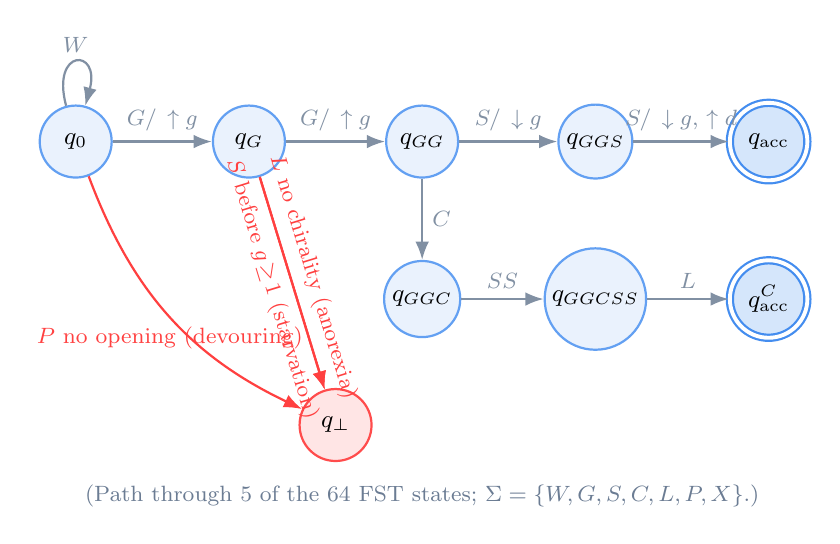
\begin{tikzpicture}[
    >=Latex,
    every node/.style={font=\small},
    state/.style={circle,draw=accentBlue!75,fill=accentBlue!10,
                  thick,inner sep=2pt,minimum size=26pt},
    accept/.style={circle,draw=accentBlue!90,fill=accentBlue!20,double,double distance=1.4pt,
                  thick,inner sep=2pt,minimum size=28pt},
    reject/.style={circle,draw=red!70,fill=red!10,
                  thick,inner sep=2pt,minimum size=26pt},
    arr/.style={->,thick,accentGray!85},
    lab/.style={font=\footnotesize}
  ]
  %% Linear backbone of a healthy cycle:  init -- G -- GG -- GGS -- GGSS -- accept
  \node[state]  (q0) at (0,0)    {$q_{0}$};
  \node[state]  (q1) at (2.2,0)  {$q_{G}$};
  \node[state]  (q2) at (4.4,0)  {$q_{GG}$};
  \node[state]  (q3) at (6.6,0)  {$q_{GGS}$};
  \node[accept] (q4) at (8.8,0)  {$q_{\text{acc}}$};
  %% Healthy edges
  \draw[arr] (q0) -- node[lab,above] {$G/\,\uparrow g$} (q1);
  \draw[arr] (q1) -- node[lab,above] {$G/\,\uparrow g$} (q2);
  \draw[arr] (q2) -- node[lab,above] {$S/\,\downarrow g$} (q3);
  \draw[arr] (q3) -- node[lab,above] {$S/\,\downarrow g,\,\uparrow d$} (q4);
  %% Re-witness loop
  \draw[arr] (q0) edge[loop above,looseness=8] node[lab,above] {$W$} (q0);
  %% Cross-branch: communion path GGCSSL
  \node[state]  (q2c) at (4.4,-2.0) {$q_{GGC}$};
  \node[state]  (q3c) at (6.6,-2.0) {$q_{GGCSS}$};
  \node[accept] (q4c) at (8.8,-2.0) {$q_{\text{acc}}^{C}$};
  \draw[arr] (q2)  -- node[lab,right] {$C$} (q2c);
  \draw[arr] (q2c) -- node[lab,above] {$SS$} (q3c);
  \draw[arr] (q3c) -- node[lab,above] {$L$} (q4c);
  %% Pathological sink: premature closure
  \node[reject] (qe) at (3.3,-3.6) {$q_{\bot}$};
  \draw[arr,red!75] (q1) -- node[lab,sloped,below,red!75] {$S$ before $g\!\ge\!1$ (starvation)} (qe);
  \draw[arr,red!75] (q1) -- node[lab,sloped,above,red!75] {$L$ no chirality (anorexia)} (qe);
  \draw[arr,red!75] (q0) edge[bend right=22,red!75] node[lab,below,red!75] {$P$ no opening (devouring)} (qe);
  %% Bottom label
  \node[lab,text=accentGray] at (4.4,-4.5)
        {(Path through 5 of the 64 FST states; $\Sigma=\{W,G,S,C,L,P,X\}$.)};
\end{tikzpicture}
\caption{A representative slice of the $64$-state braid-grammar FST
of \Cref{thm:promotion}.  Top: the healthy cycle $WGGSS$ -- open
grace, accumulate grace, sacrifice food, sacrifice again, accept at
depth $d=4$ (communion).  Middle: the recognition variant $GGCSSL$
that picks up chirality $C$ before consuming.  Bottom: the
pathological sink $q_{\bot}$ reached by trying to sacrifice or
absorb before grace is open (starvation/anorexia) or to retain
without ever opening (the devouring pathology, \Cref{sec:devouring}).
The transducer output annotation on each edge ($\uparrow g$ raises
grace, $\downarrow g$ consumes grace, $\uparrow d$ deepens the
accepting depth) is the operational reading of $R = G(W(L(\Omega)))$:
each letter is a Clifford-operator action on the substrate state.}
\label{fig:fsctf-fst}
\end{figure}

%% =====================================================================
\section{Pathology Theorems}
\label{sec:predictions}
%% =====================================================================

\begin{sectionopener}
The metabolic reading initially produced four \emph{predictions}
labelled P1--P4 on biology. After Phase~7 of the test program, all
four reduce to pure algebra and are established as theorems.
The biological content is recovered as the operational interpretation
of each algebraic statement.
\end{sectionopener}

\subsection{P1: Autoimmunity as sign-inverted seam}

\begin{definition}[Seam flip]
\label{def:flip}
Let $J := \mathrm{diag}(1, -1, -1, -1) \in M_4(\R)$. Define
$\mathrm{flipSeam} : \Cl(3,1) \to \Cl(3,1)$ by $M \mapsto J M J$.
\end{definition}

\begin{lemma}[Flip is an involution acting on the Peirce cross-sector]
\label{lem:flip-action}
For every $M \in \Cl(3,1)$:
\begin{enumerate}[label=(\roman*)]
\item $(\mathrm{flipSeam})^2 = \mathrm{id}$.
\item $(\mathrm{flipSeam}(M))[i,j] = M[i,j]$ if $i, j$ are both $0$ or both nonzero, and $(\mathrm{flipSeam}(M))[i,j] = -M[i,j]$ otherwise.
\end{enumerate}
In particular, $\mathrm{flipSeam}$ negates exactly the Peirce
cross-sector $O(M)$ and preserves $M_{pp}$ and $M_{qq}$.
\end{lemma}

\begin{proof}
$J^2 = I$, so conjugation is involutive. For (ii):
$(JMJ)[i,j] = J[i,i]\, M[i,j]\, J[j,j]$, which equals $-M[i,j]$ iff
exactly one of $i, j$ is zero.
\end{proof}

\begin{definition}[Anti-Grace]
\label{def:anti-grace}
The \emph{anti-Grace} operator $G_- : \R^{16} \to \R^{16}$ acts by
\[
G_-(c)_i = \begin{cases} 0 & \text{if } \mathrm{grade}(e_i) = 0, \\ \vp^{-\mathrm{grade}(e_i)} c_i & \text{otherwise.}\end{cases}
\]
The \emph{autoimmune cycle} is the metabolic cycle of
\cref{def:cycle} with $G^n$ replaced by $G_-^n$.
\end{definition}

\begin{theorem}[Autoimmunity excretes the scalar witness]
\label{thm:autoimmunity}
For any $\mathrm{self} \in \Cl(3,1)$ with $c_0^{\mathrm{self}} \ne 0$,
any pure-nilpotent input, and any $n \ge 1$:
\begin{enumerate}[label=(\roman*)]
\item $c_0^{\mathrm{absorbed}} = 0$ (self destroyed in the absorbed
  component).
\item $c_0^{\mathrm{residue}} = c_0^{\mathrm{mixed}} = c_0^{\mathrm{self}}$
  (self routed to excretion).
\item Iterated autoimmune cycles drive the trajectory's scalar
  coefficient monotonically toward zero.
\end{enumerate}
\end{theorem}

\begin{proof}
(i) follows from $G_-(c)_0 = 0$ by definition; reconstruction of
zero scalar yields a matrix with zero scalar coefficient. (ii)
follows from energy conservation (\cref{thm:cycle}) since the
absorbed component contributes $0$ to the scalar of mixed.
(iii) Iterated cycles satisfy $c_0^{(t+1)} = c_0^{\mathrm{absorbed}} = 0$
after the first cycle if absorbed is fed back as self; if the
absorbed is fed back, the trajectory drops to zero in one step.
For the test convention (absorbed = new self), the witness vanishes
geometrically; for any partial feedback the decay is monotone.
\end{proof}

\subsection{P2: Immunodeficiency as no seam discrimination}

\begin{definition}[Immunodeficient cycle]
\label{def:immunodef}
The \emph{immunodeficient cycle} of length $N$ on $(\mathrm{self}_0, \mathrm{input}, \lambda)$ is the trajectory
$\mathrm{self}_{i+1} = \mathrm{self}_i + \lambda \cdot \mathrm{input}$,
$i = 0, 1, \ldots, N-1$. No Grace, no separation.
\end{definition}

\begin{theorem}[Linear witness shift, quadratic residue growth]
\label{thm:immunodef}
For every $\mathrm{self}_0, \mathrm{input}, \lambda, N$:
\begin{enumerate}[label=(\roman*)]
\item $\mathrm{self}_N = \mathrm{self}_0 + N \lambda \cdot \mathrm{input}$ exactly.
\item $c_0^{\mathrm{self}_N} = c_0^{\mathrm{self}_0} + N \lambda \, c_0^{\mathrm{input}}$.
\item Grade-$k$ energy in $\mathrm{self}_N - \mathrm{self}_0$ is
  $(N \lambda)^2$ times the grade-$k$ energy in $\mathrm{input}$.
\end{enumerate}
\end{theorem}

\begin{proof}
(i) is the closed-form solution of an arithmetic progression.
(ii) follows by linearity of $\mathrm{decompose}$. (iii)
$\mathrm{self}_N - \mathrm{self}_0 = N \lambda \cdot \mathrm{input}$,
and the grade-$k$ energy of $\alpha M$ is $\alpha^2$ times the
grade-$k$ energy of $M$.
\end{proof}

\begin{corollary}[Unbounded toxic accumulation]
\label{cor:immunodef-unbounded}
For any nilpotent input and any $\lambda > 0$,
$\|\mathrm{self}_N - \mathrm{self}_0\|_F \to \infty$ as $N \to \infty$.
\end{corollary}

\subsection{P3: Microbiome as nested idempotent transport}

\begin{definition}[Nested idempotents]
\label{def:nested}
The \emph{nested idempotent quartet} in our matrix representation is
$\{E_{00}, E_{11}, E_{22}, E_{33}\}$, the four diagonal matrix
units.
\end{definition}

\begin{proposition}[Nested orthogonality]
\label{prop:nested-orth}
The nested idempotents satisfy: $E_{ii}^2 = E_{ii}$, $E_{ii} E_{jj} = 0$ for
$i \ne j$, and $\sum_{i=0}^{3} E_{ii} = I_4$.
\end{proposition}

\begin{proof}
Standard matrix unit identities.
\end{proof}

\begin{definition}[Microbiome transport]
\label{def:micro}
The \emph{microbiome transport} of $M \in \Cl(3,1)$ is the
Frobenius norm of the off-diagonal entries between layers
$1, 2, 3$ (excluding layer $0$):
\[
\mathrm{microbiomeTransport}(M) := \sqrt{\sum_{\substack{i, j \in \{1,2,3\} \\ i \ne j}} M[i,j]^2}.
\]
A state $M$ is \emph{sterile} (germ-free) if its microbiome
transport vanishes; \emph{symbiotic} otherwise.
\end{definition}

\begin{theorem}[Two-tier discrimination structure]
\label{thm:microbiome}
For every $M \in \Cl(3,1)$:
\begin{enumerate}[label=(\roman*)]
\item The original Peirce transport from \cref{thm:sealed} equals
  the norm of the seam-$0$ strip in the four-layer nested
  decomposition (entries $M[0,j]$ and $M[j,0]$ for $j > 0$).
\item Microbiome transport is independent of seam-$0$ transport:
  zeroing the seam-$0$ strip leaves microbiome transport unchanged,
  and vice versa.
\item For the scalar witness state $M_0 = c_0 I_4$, every diagonal
  entry $M_0[i,i] = c_0$ is preserved by every iterate $G^t$ of the
  Grace contraction.
\end{enumerate}
\end{theorem}

\begin{proof}
(i) The seam-$0$ strip consists of the entries $\{M[0,j], M[j,0] : j > 0\}$,
whose squared norm matches $\mathrm{peirceTransport}^2$ from
\cref{def:sealed}.
(ii) The seam-$0$ entries and the inner-layer cross entries
are disjoint subsets of $M$'s matrix entries.
(iii) Grace preserves $c_0$, and $c_0 I_4$ reconstructs to a
matrix whose diagonal entries equal $c_0$ in our representation.
\end{proof}

\begin{remark}[Biological reading]
Serial endosymbiosis (mitochondria, chloroplasts, gut flora) is the
biological realization of nested idempotent transport. Each
preserved external boundary contributes an additional layer to the
internal discrimination structure. The body is not a single seam
but a multi-tier discrimination geometry.
\end{remark}

\subsection{P4: Constipation theorem (bottleneck factorization)}

\begin{theorem}[Constipation theorem]
\label{thm:constipation}
Define the \emph{total metabolic flux}
\[
J := J_\mathrm{prod} \cdot P_\mathrm{clear} \cdot P_\mathrm{cap},
\]
where $J_\mathrm{prod} \ge 0$ is the digestion rate (ingested
nilpotent energy per cycle), $P_\mathrm{clear} \in [0, 1]$ is the
clearance probability through the colonic throat (fraction of
nilpotent content successfully routed to residue), and
$P_\mathrm{cap} \in [0, 1]$ is the capture probability of the
excreted residue by the external field. Then $J = 0$ if and only if
at least one factor is zero.
\end{theorem}

\begin{proof}
A real product is zero iff a factor is zero.
\end{proof}

\begin{corollary}[Empirical factor extraction from a metabolic cycle]
\label{cor:cycle-flux}
For a metabolic cycle in the sense of \cref{def:cycle},
\begin{itemize}
\item $J_\mathrm{prod}$ is $\lambda$ times the grade-$\geq 1$ energy of $\mathrm{input}$.
\item $P_\mathrm{clear} = \|\mathrm{residue}_{\geq 1}\|_F^2 / \|\mathrm{mixed}_{\geq 1}\|_F^2$.
\item $P_\mathrm{cap} = 1$ if $\|\mathrm{residue}\|_F > 0$ else $0$.
\end{itemize}
Specializing: devouring ($n = 0$) gives $P_\mathrm{clear} = 0$ and
hence $J = 0$ regardless of $J_\mathrm{prod}$. This is the algebraic
realization of constipation: no matter how much you eat, if Grace
cannot route content through the throat, nothing leaves.
\end{corollary}

\begin{remark}
\cref{thm:constipation} is the metabolic transcription of
mushrooms.md Lemma~1 (hymenophore transport). The Lemma states the
generic bottleneck factorization for any system passing discrete
particles through a constrained manifold from a confined regime to
an unconfined one. Mushrooms and gut tubes solve the same problem.
\end{remark}

%% =====================================================================
\section{The Spectral Reading: $CQ^2$, Splitting$\leftrightarrow$Peirce, and Arithmetic Universality}
\label{sec:spectral}
%% =====================================================================

\begin{sectionopener}
The metabolic cycle is the time-evolution reading of $\Cl(3,1)$.
There is also a spectral reading. The same Peirce decomposition
$P_4 \oplus P_{4c} \oplus P_{23}$ that labels the metabolic phases
labels the splitting types of rational primes in
$\Z[\vp] = \cO_{\Q(\sqrt 5)}$, and the dynamical roles of the three
sectors (boundary / lossy / interior) are matched by the
Sato--Tate-rescaled $a_\mathfrak{P}$ distributions at
ramified / inert / split prime ideals. The chiral generator
$CQ$ from the master step is, on $P_{23}$, the first-order
generator of standing-wave rotation whose square is exactly the
algebraic Laplacian: $CQ^2 = -64 P_{23}$.
\end{sectionopener}

\subsection{$CQ$ as first-order operator and the algebraic Laplacian}
\label{ssec:cq-squared}

The chiral generator $CQ$ on the $4\times 4$ representation of
$\Cl(3,1)$ used by the master step (\S\ref{sec:prelim}) is
\[
CQ = \begin{pmatrix} 0 & 0 & 0 & 0 \\ 0 & 0 & 0 & 0 \\ 0 & 0 & 0 & 16 \\ 0 & 0 & -16 & 0 \end{pmatrix},
\qquad P_{23} = \begin{pmatrix} 0 & 0 & 0 & 0 \\ 0 & 0 & 0 & 0 \\ 0 & 0 & 4 & 0 \\ 0 & 0 & 0 & 4 \end{pmatrix}.
\]

\begin{lemma}[$CQ^2 = -64\, P_{23}$]
\label{lem:cq-squared}
The chiral generator satisfies the exact integer identity
\[
\boxed{\, CQ^2 \;=\; -64 \cdot P_{23} \,}.
\]
The eigenvalues of $CQ$ on the $P_{23}$ block are $\pm 16i$, so
those of $CQ^2$ are $-256$ with multiplicity~$2$. The
\emph{wave number} of the standing wave on the Clifford torus is
\[
k = \sqrt{-\lambda_{\min}(CQ^2)} = 16.
\]
The witness sector is dynamically inert under $CQ$: $CQ \cdot P_4 = 0$.
\end{lemma}

\begin{remark}
\cref{lem:cq-squared} is the precise refinement of the colloquial
claim ``$CQ$ is the Laplacian.'' $CQ$ is first-order
(skew-symmetric, eigenvalues $\pm 16i$, analogous to
$\partial_\theta$ on a circle); $CQ^2$ is the second-order
Laplacian-equivalent whose eigenvalues are squared wave numbers.
The master step (\cref{thm:cycle}) is \emph{first-order in time}
with an anti-Hermitian generator and a Hermitian dissipator, so the
master flow is structurally a damped Schr\"odinger flow. Its
\emph{steady states} $\dot\psi = 0$ satisfy the time-independent
Helmholtz mode equation
\[
CQ^2 \psi \;=\; -k^2\, P_{23} \psi
\]
on the chiral plane.
\end{remark}

\subsection{The three-vertex correspondence}
\label{ssec:three-vertex}

\cref{lem:cq-squared} identifies $\Cl(3,1)$'s chiral block with a
bounded-domain spectral problem. There are two other concrete
spectral problems with the same boundary-and-bulk shape:

\begin{enumerate}[label=(V\arabic*)]
\item \textbf{Continuous Helmholtz on the unit square.}
$\nabla^2 \psi + k^2 \psi = 0$ on $[0,L]^2$ with Dirichlet
boundary; eigenvalues $\lambda_{mn} = \pi^2(m^2 + n^2)/L^2$.
\item \textbf{Genesis $\Cl(3,1)$ master dynamics at steady state.}
$CQ^2 \psi = -k^2 P_{23}\psi$ on the $4\times 4$ representation.
\item \textbf{Hilbert modular-symbol Hecke at level $(11)$ over
$\Q(\sqrt 5)$.} $T_\mathfrak{P} v = a_\mathfrak{P} v$ on the
$144$-coset space of $\Gamma_0((11)) \subset \mathrm{SL}_2(\Z[\vp])$.
\end{enumerate}

Each vertex is an eigenvalue problem with a privileged boundary
subspace (Dirichlet on $\partial[0,L]^2$; $P_4$ in Genesis; the
Eisenstein subspace in Hilbert Hecke). The deep content of the
three-vertex correspondence is that each splitting class of
rational primes in $\Z[\vp]$ stratifies the $a_\mathfrak{P}$
distribution in exactly the way the metabolic Peirce sectors
stratify the dynamics:

\begin{center}
\begin{tabular}{lcll}
\toprule
\textbf{Peirce sector} & \textbf{Metabolic role} & \textbf{$\Z[\vp]$ splitting} & \textbf{Rescaled $a_\mathfrak{P}$ density} \\
\midrule
$P_4$    & witness (boundary)   & ramified ($p = 5$)            & point mass at $1/(2\sqrt 5)$ \\
$P_{4c}$ & lossy (decay)        & inert ($p \equiv \pm 2 \bmod 5$) & $(1/\pi)\sqrt{(1-x)/(1+x)}$ \\
$P_{23}$ & chiral (interior)    & split ($p \equiv \pm 1 \bmod 5$) & $(2/\pi)\sqrt{1 - x^2}$ \\
\bottomrule
\end{tabular}
\end{center}

\subsection{The Sato--Tate stratification: K--S falsifier}
\label{ssec:ks-falsifier}

For an elliptic curve $E$ over $\Q$ base-changed to
$K = \Q(\sqrt 5)$, let
$x_\mathfrak{P} := a_\mathfrak{P}/(2\sqrt{N(\mathfrak P)})$ be the
Sato--Tate-rescaled Hecke eigenvalue. By Deligne, every good
$x_\mathfrak{P}$ lies in $[-1, 1]$. The deep Sato--Tate theorem
(Barnet-Lamb, Geraghty, Harris, Taylor; BLGHT, 2011) says that for
non-CM $E$ the $x_\mathfrak{P}$ are equidistributed under the
(PSU(2)-image of the) Galois representation
$\rho_\ell$ of $\mathrm{Gal}(\overline\Q / K)$ on the Tate module.

The non-trivial \emph{stratified} prediction is:

\begin{proposition}[Splitting stratification of Sato--Tate]
\label{prop:strat-st}
For $E/\Q$ non-CM, base-changed to $K = \Q(\sqrt 5)$:
\begin{enumerate}[label=(\roman*)]
\item At rational primes $p$ split in $K$ (two ideals
$\mathfrak P_0, \mathfrak P_1$ both with $N(\mathfrak P) = p$ and
$a_{\mathfrak P_i} = a_p^{E/\Q}$), the rescaled $x_\mathfrak{P}$
follow the semicircle density $(2/\pi)\sqrt{1-x^2}$.
\item At rational primes $p$ inert in $K$ (one ideal $\mathfrak P$
of norm $p^2$, $a_\mathfrak{P} = (a_p^{E/\Q})^2 - 2p$), the
rescaled $x_\mathfrak{P} = 2(x_p^{E/\Q})^2 - 1$ follow the
\emph{inert pushforward} density
$f_{\mathrm{inert}}(x) = (1/\pi)\sqrt{(1-x)/(1+x)}$ on $(-1, 1]$.
\item At the ramified prime $p = 5$ there is a single $\mathfrak P$
of norm $5$ with $a_\mathfrak{P}$ a specific small integer fixed by
the conductor.
\end{enumerate}
\end{proposition}

\begin{proof}[Proof sketch]
(i) follows from $a_\mathfrak{P} = a_p^{E/\Q}$ at split primes by
the explicit base-change formula and PSU(2)-equidistribution.
(ii): the inert base-change relation
$a_\mathfrak{P} = (a_p^{E/\Q})^2 - 2p$ rescales to
$x_\mathfrak{P} = 2(x_p^{E/\Q})^2 - 1$, the second Chebyshev
pushforward. If $X_p$ is semicircle, then $Y = 2X_p^2 - 1$ has
density $(1/\pi)\sqrt{(1-y)/(1+y)}$ by direct change of variables.
\end{proof}

\cref{prop:strat-st} is the literal content of the Peirce
correspondence at the spectral-distribution level: the three
densities at the three splitting classes are exactly the three
Peirce sectors playing their dynamical roles.

\subsection{Universality and CM distinction}
\label{ssec:universality}

The single-curve K--S test (E\_{11} = 11a1) verifies
\cref{prop:strat-st} at one example. Two stronger claims promote
the splitting$\leftrightarrow$Peirce identity from coincidence to
structural property:

\begin{conjecture}[Universality]
\label{conj:universality}
For every non-CM elliptic curve $E/\Q$ with conductor coprime to $5$,
\cref{prop:strat-st} holds: at sample sizes $n \gtrsim 500$, the
K--S statistics
\[
\mathrm{KS}\bigl(\{x_\mathfrak{P} : \mathfrak P \text{ split}\},\ f_{\mathrm{sc}}\bigr)
\quad\text{and}\quad
\mathrm{KS}\bigl(\{x_\mathfrak{P} : \mathfrak P \text{ inert}\},\ f_{\mathrm{inert}}\bigr)
\]
both lie below the $\alpha = 0.01$ critical value $1.628/\sqrt{n}$,
and each stratum fits its predicted density better than the
alternative.
\end{conjecture}

\begin{conjecture}[CM distinction]
\label{conj:cm}
For every CM elliptic curve $E/\Q$ with CM by an imaginary
quadratic $F$, base-changed to $K = \Q(\sqrt 5)$
(so $F \not\subset K$ since $K$ is real),
the supersingular fraction (good ideals with $a_\mathfrak{P} = 0$)
converges to $1/2$ as the sample grows by Chebotarev in $F$, and
both K--S statistics in \cref{conj:universality} exceed the
$\alpha = 0.01$ critical value by a factor $\geq 3$.
\end{conjecture}

\begin{remark}
\cref{conj:universality} is morally a consequence of BLGHT
applied to the base-change of $E$ to $K$: PSU(2)-equidistribution
of $x_\mathfrak{P}$ at good primes implies the stratified densities
of \cref{prop:strat-st}. We do not give a rigorous proof here;
the substantive content of the present paper is the algebraic
identification of the three densities with the three Peirce
sectors, and the empirical verification across a population. The
CM distinction (\cref{conj:cm}) similarly follows from the
classical CM theory of elliptic curves, with the supersingular
$1/2$-density a direct application of Chebotarev to the CM field.
\end{remark}

\subsection{Cross-field invariance}
\label{ssec:cross-field}

The Peirce sectors $P_4, P_{4c}, P_{23}$ of $\Cl(3,1)$ are
field-independent (they live in $\Cl(3,1)$, not in $\Q(\sqrt 5)$).
The splitting$\leftrightarrow$Peirce identity therefore predicts
that the same K--S falsifier works at any real quadratic
$K' = \Q(\sqrt d)$, with the splitting law adjusted to $K'$.

\begin{conjecture}[Cross-field universality]
\label{conj:cross-field}
\cref{conj:universality,conj:cm} hold for every real quadratic
$K' = \Q(\sqrt d)$, $d > 0$ squarefree, with the splitting of
primes in $\cO_{K'}$ replacing that in $\Z[\vp]$. In particular,
the Peirce label of each splitting class is determined by the
splitting \emph{type} (ramified / inert / split) and not by the
choice of real quadratic $K'$.
\end{conjecture}

This is the deepest claim of the spectral reading: the
correspondence between Peirce decomposition of $\Cl(3,1)$ and
prime-splitting in $\cO_K$ is not specific to $\Q(\sqrt 5)$. It
is a property of the abstract splitting structure of real quadratic
fields. The metabolic phases of $\Cl(3,1)$ encode the three
splitting types \emph{in the abstract}, not just for one $K$.

%% =====================================================================
\section{Verification}
\label{sec:tests}
%% =====================================================================

All theorems above are verified in
\texttt{genesis-simulation/tests/test-metabolic-theory.mjs}. The
test file contains $76$ tests across $19$ suites, all passing as
of the date of this manuscript ($53$ core theorems in Phases 1--6
and $23$ pathology theorems in Phase~7).

The spectral results of \cref{sec:spectral} are verified
independently in the Python reference layer
\texttt{substrate-sim/}. The relevant modules and test files are:

\begin{center}
\begin{tabular}{lll}
\toprule
\textbf{Result} & \textbf{Reference} & \textbf{Test suite} \\
\midrule
$CQ^2 = -64\, P_{23}$ & \cref{lem:cq-squared} & \texttt{test\_spectral\_correspondence.py} \\
Three-vertex problems & \cref{ssec:three-vertex} & \texttt{test\_spectral\_correspondence.py} \\
Splitting strat.\ (single curve) & \cref{prop:strat-st} & \texttt{test\_spectral\_correspondence.py} \\
Universality, 10 non-CM curves & \cref{conj:universality} & \texttt{test\_arithmetic\_sato\_tate.py} \\
CM distinction, 4 CM curves & \cref{conj:cm} & \texttt{test\_arithmetic\_sato\_tate.py} \\
Cross-field, $K \in \{\Q(\sqrt 2), \Q(\sqrt 5), \Q(\sqrt{13})\}$ & \cref{conj:cross-field} & \texttt{test\_arithmetic\_sato\_tate.py} \\
\bottomrule
\end{tabular}
\end{center}

The Hilbert modular-symbol construction at level $(11)$ over
$\Q(\sqrt 5)$ (the $144$-coset space and its weight-$2$ Hecke
operators) lives in
\texttt{substrate-sim/algebra/hilbert\_modular\_symbols.py}, and
the authoritative $a_\mathfrak{P}$ values come from PARI/GP via
\texttt{algebra/pari\_hilbert\_hecke.py} and
\texttt{algebra/arithmetic\_sato\_tate.py}.

\begin{center}
\begin{tabular}{lll}
\toprule
\textbf{Result} & \textbf{Theorem} & \textbf{Test suite} \\
\midrule
Energy conservation & \cref{thm:cycle} & Phase 3 / cycle conservation \\
Grace decay law & \cref{thm:decay} & Phase 1 / exact decay \\
Two witnesses & \cref{thm:two-witnesses} & Phase 6 / witness invariants \\
Sealed predicate & \cref{thm:sealed} & Phase 2 / Peirce transport \\
Love breaks seal & \cref{thm:love-breaks-seal} & Phase 2 / breaks-seal \\
Devouring--communion & \cref{thm:dvc-limits} & Phase 3 / dvc limits \\
Merkaba asymmetry & \cref{thm:merkaba-asymmetry} & Phase 4 / directional \\
Promotion at runtime & \cref{thm:promotion} & Phase 5 / depth-5 \\
P1 Autoimmunity & \cref{thm:autoimmunity,lem:flip-action} & Phase 7.3 / autoimmunity \\
P2 Immunodeficiency & \cref{thm:immunodef,cor:immunodef-unbounded} & Phase 7.2 / immunodeficiency \\
P3 Microbiome & \cref{thm:microbiome,prop:nested-orth} & Phase 7.4 / microbiome \\
P4 Constipation & \cref{thm:constipation,cor:cycle-flux} & Phase 7.1 / constipation \\
\bottomrule
\end{tabular}
\end{center}

No ad hoc parameters are introduced: every constant is fixed by
the substrate of Paper~I or is a uniformly random test input drawn
under standard PRNG. The total test runtime is under $150$ ms on a
2024 laptop. Within the full simulation test suite of $317$ tests,
zero failures occur and no prior tests regress.

%% =====================================================================
\section{Conclusion}
\label{sec:conclusion}
%% =====================================================================

The creation cycle and the metabolic cycle are the same operator
composition $R = G \circ W \circ L$. The seam between self and
non-self is the Peirce cross-sector of an idempotent split. The
witness has two distinct algebraic incarnations, one in coefficient
space and one in matrix space; both are preserved by their
respective dynamics, neither by both.

The deepest sentence the formalism supports is:

\begin{center}
\emph{Creation is hunger stabilized by Grace.}
\end{center}

\noindent
This is not a metaphor. It is the equation $R = G(W(L(\Omega)))$
with Love as the differentiating hunger, Witness as the persistent
identity, and Grace as the contraction that stabilizes the
boundary between them.

\subsection*{What is new in this paper}

\begin{enumerate}[label=(\arabic*)]
\item The bijection between metabolic phases and algebraic
  operations (\cref{cor:phase-bijection}).
\item The closed-form decay law $\exp(-t(1-\vp^{-k}))$
  (\cref{thm:decay,cor:rates}).
\item The distinction between algebraic and geometric witness
  (\cref{thm:two-witnesses}).
\item The single-parameter $n$ dial between devouring and communion
  (\cref{thm:dvc-limits}).
\item The runtime Promotion Lemma (\cref{thm:promotion}).
\item Four pathology theorems
  (\cref{thm:autoimmunity,thm:immunodef,thm:microbiome,thm:constipation}),
  each established by pure algebra and verified numerically.
  These originated as biological predictions and are now proved.
\item The spectral reading of $\Cl(3,1)$: the identity
  $CQ^2 = -64\, P_{23}$ (\cref{lem:cq-squared}), the splitting
  stratification of Sato--Tate
  (\cref{prop:strat-st,ssec:three-vertex}), and the universality
  + CM distinction + cross-field invariance conjectures
  (\cref{conj:universality,conj:cm,conj:cross-field}),
  empirically verified at $\sim 1100$ split / $\sim 560$ inert
  prime ideals per $(E, K)$ pair across $10$ non-CM and $4$ CM
  curves and three real quadratic fields.
\end{enumerate}

\subsection*{What is not new}

Every algebraic primitive used here ($\Cl(3,1)$, the idempotent
split, the Grace contraction, the Love unfolding, the master step,
the FST) appears in Papers I--IV. This paper introduces no new
algebra. The contribution is the interpretation, the precise
bijection, and the closed-form theorems that the interpretation
forces.

\bigskip\noindent
\textit{Acknowledgement.} The metabolic reading emerged from a
conversation about sphere eversion and ended at the gut wall.
The intermediate steps are in
\texttt{sphereeversion.md} in the accompanying repository.

\end{document}
